%%% Template originaly created by Karol Kozioł (mail@karol-koziol.net) and modified for ShareLaTeX use

\documentclass[a4paper,11pt]{article}

\usepackage[T1]{fontenc}
\usepackage[utf8]{inputenc}
\usepackage{graphicx}
\usepackage{xcolor}
 \usepackage{tgtermes}

 \usepackage[
 pdftitle={Math Assignment},
 pdfauthor={Joe Doe, Some University},
 colorlinks=true,linkcolor=blue,urlcolor=blue,citecolor=blue,bookmarks=true,
 bookmarksopenlevel=2]{hyperref}
\usepackage{amsmath,amssymb,amsthm,textcomp}
\usepackage{enumerate}
\usepackage{multicol}
\usepackage{tikz}

\usepackage{geometry}
\geometry{total={210mm,297mm},
left=25mm,right=25mm,%
bindingoffset=0mm, top=20mm,bottom=20mm}


\linespread{1.3}

\newcommand{\linia}{\rule{\linewidth}{0.5pt}}

% custom theorems if needed
\newtheoremstyle{mytheor}
    {1ex}{1ex}{\normalfont}{0pt}{\scshape}{.}{1ex}
    {{\thmname{#1 }}{\thmnumber{#2}}{\thmnote{ (#3)}}}

\theoremstyle{mytheor}
\newtheorem{defi}{Definition}
\usepackage[ruled, vlined, linesnumbered,lined,boxed,commentsnumbered]{algorithm2e}
\usepackage[parfill]{parskip}
\makeatletter

\setlength\parindent{0pt}
% custom footers and headers
\usepackage{fancyhdr,lastpage}


%%%----------%%%----------%%%----------%%%----------%%%

\begin{document}

\title{CSE 250B: Machine Learning}

\author{Sai Bi}

\date{\today}

\maketitle

\section*{Problem 1}
\subsection*{a}
The parameters for the bivariate Gaussian is:
\begin{align}
	\begin{split}
	\mu &= (\mu_x, \mu_y) \\
	    &= (2, 2)  \\
	\sum &= \begin{bmatrix}
				1  & -0.5 \\
				-0.5 & 0.5 
			\end{bmatrix}
	\end{split}
\end{align}

\subsection*{b}
The parameters for the bivariate Gaussian is:
\begin{align}
\begin{split}
\mu &= (\mu_x, \mu_y) \\
&= (1, 1)  \\
\sum &= \begin{bmatrix}
1  & 1 \\
1 & 1 
\end{bmatrix}
\end{split}
\end{align}

\section*{Problem 2}
\subsection*{a}
See Figure~\ref{fig:2a}
\begin{figure}[t]
	\centering{
	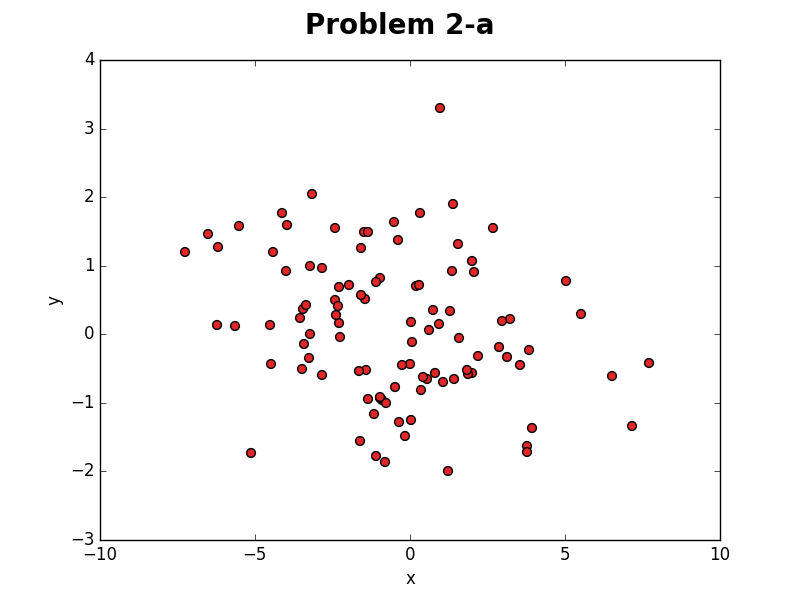
\includegraphics[width = \textwidth]{./code/2-a.png}
	}
	\label{fig:2a}
\end{figure}

\subsection*{b}
See Figure~\ref{fig:2b}
\begin{figure}[t]
	\centering{
		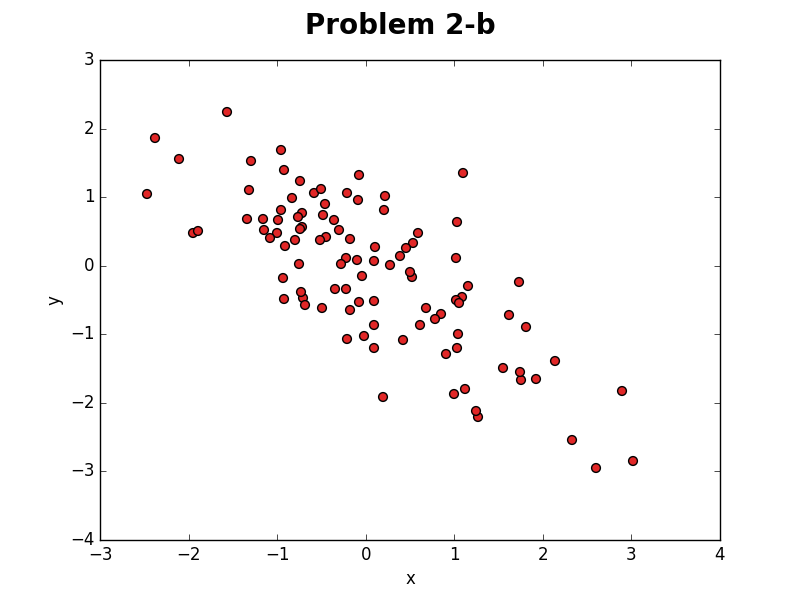
\includegraphics[width = \textwidth]{./code/2-b.png}
	}
	\label{fig:2b}
\end{figure}


\section*{Problem 3}
\subsection*{a}
See Figure~\ref{fig:3}
\begin{figure}[t]
	\centering{
		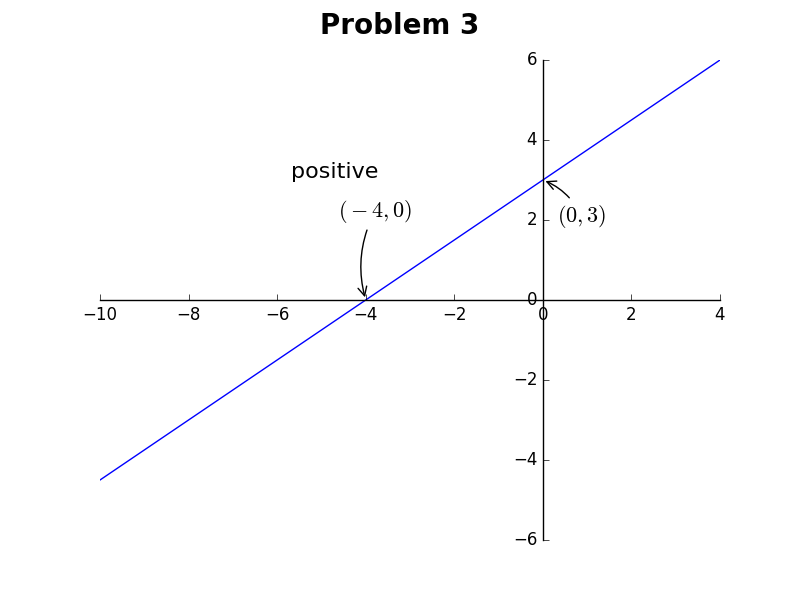
\includegraphics[width = \textwidth]{./code/3.png}
	}
	\label{fig:3}
\end{figure}

\section*{Problem 4}
\subsection*{a}
Check whether the number of distinct eigenvalues $\lambda$ is equal to $p$, and
if yes, $\sum$ is invertible, otherwise not.

\subsection*{b}
The eigenvalues of $\sum + c I$ are $(\lambda_1 + c), ... , (\lambda_p + c)$.
The eigenvectors of $\sum + c I$ are $u_1, ..., u_p$.

\subsection*{c}







\end{document}
